\documentclass[12pt]{article}
\usepackage[left=1cm, right=1cm, top=2cm,bottom=1.5cm]{geometry} 

\usepackage[parfill]{parskip}
\usepackage[utf8]{inputenc}
\usepackage[T2A]{fontenc}
\usepackage[russian]{babel}
\usepackage{enumitem}
\usepackage[normalem]{ulem}
\usepackage{amsfonts, amsmath, amsthm, amssymb, mathtools}

\usepackage{fancyhdr}
\pagestyle{fancy}
\renewcommand{\headrulewidth}{1.5pt}
\renewcommand{\footrulewidth}{1pt}

\usepackage{graphicx}
\usepackage[figurename=Рис.]{caption}
\usepackage{subcaption}
\usepackage{float}

%%Наименование папки откуда забирать изображения
\graphicspath{ {./images/} }

%%Изменение формата для ввода доказательства
\renewcommand{\proofname}{$\square$  \nopunct}
\renewcommand\qedsymbol{$\blacksquare$}

\addto\captionsrussian{%
	\renewcommand{\proofname}{$\square$ \nopunct}%
}
%% Римские цифры
\newcommand{\RN}[1]{%
	\textup{\uppercase\expandafter{\romannumeral#1}}%
}


\theoremstyle{definition}
\newtheorem{defn}{Опр:}
\newtheorem{rem}{Rm:}
\newtheorem{prop}{Утв.}
\newtheorem{exrc}{Упр.}
\newtheorem{lemma}{Лемма}
\newtheorem{theorem}{Теорема}
\newtheorem{corollary}{Следствие}

\newenvironment{cusdefn}[1]
{\renewcommand\thedefn{#1}\defn}
{\enddefn}



\DeclareRobustCommand{\divby}{%
	\mathrel{\text{\vbox{\baselineskip.65ex\lineskiplimit0pt\hbox{.}\hbox{.}\hbox{.}}}}%
}


\newcommand{\smallerrel}[1]{\mathrel{\mathpalette\smallerrelaux{#1}}}
\newcommand{\smallerrelaux}[2]{\raisebox{.1ex}{\scalebox{.75}{$#1#2$}}}

\newcommand{\smallin}{\smallerrel{\in}}
\newcommand{\smallnotin}{\smallerrel{\notin}}



\begin{document}
	\lhead{Математический анализ - I}
	\chead{Шапошников С.В.}
	\rhead{Лекция - 10}


\begin{defn}
	Последовательность $\{a_n\}$ \uwave{фундаментальна} или \uwave{удовлетворяет условию Коши}, если $$\forall \varepsilon > 0,\, \exists \, N \in \mathbb{N} \colon \forall n, m > N, \, |a_n - a_m| < \varepsilon$$
\end{defn}

Можно доказать, что из критерия Коши следует принцип вложенных отрезков. Из принципа вложенных отрезков и аксиомы Архимеда следует аксиома полноты (без доказательства).

Свойство фундаментальности эквивалентно сходимости последовательности. Можно придумать пример, где критерий Коши будет выполнятся, но без аксиомы Архимеда это множество не будет похоже на множество вещественных чисел.

\begin{prop}
	Если последовательность $a_n$ сходится, то $a_n$ - фундаментальна.
\end{prop}

\begin{proof}
	Пусть $\lim\limits_{n\to \infty} a_n = a$ по определению: $\forall \varepsilon > 0,\, \exists \, N \in \mathbb{N} \colon \forall n > N, \, |a_n - a| < \varepsilon$.
	
	Пусть $m > N$ и $n > N$ тогда по неравенству треугольника $|a_m - a_n| \leq |a_m - a| + |a_n - a| < 2 \varepsilon \Rightarrow$ выполняется условие Коши, так как константа не важна.
\end{proof}

\begin{prop}
	Если последовательность $a_n$ фундаментальна, то она ограничена.
\end{prop}
Доказательство будет аналогично тому, что было для ограниченных последовательностей: в интервале вокруг предела - бесконечно много точек последовательности, возьмем больший интервал покрывающий оставшиеся члены последовательнсти.
\begin{figure}[H]
	\centering
	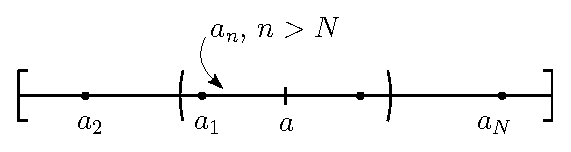
\includegraphics[width=0.35\textwidth]{10_1.eps}
	\caption{Идея доказательства}
	\label{10_1}
\end{figure}


\begin{proof}
	Возьмем $\varepsilon = 1$, тогда $\exists \, N \colon \forall n, m > N, \, |a_n - a_m| < 1$. $S = \min \{a_1, \dotsc, a_N\}$, $L = \max\{a_1, \dotsc, a_N\}$, как взять отрезок, который их будет содержать?
	
	\begin{figure}[H]
		\centering
		\includegraphics[width=0.27\textwidth]{10_2.eps}
		\caption{Отрезок покрывающий последовательность}
		\label{10_2}
	\end{figure}
	
	Возьмем отрезок $[\min\{S, a_{N+1} -1\}, \max\{L,a_{N+1}+1\}]$. В этом отрезке лежат все $a_n$.
\end{proof}

\begin{prop}
	Если последовательность $a_n$ фундаментальна и существует подпоследовательность, такая что $a_{n_k} \colon a_{n_k} \to a$, то $a_n \to a$.
\end{prop}

\begin{proof}
	$\forall \varepsilon > 0, \exists \, N \colon \forall n,m > N, \, |a_n - a_m| < \varepsilon$, пусть $k > N \Rightarrow n_k > N \Rightarrow m = n_k, \, |a_n - a_{n_k}| < \varepsilon, \, \forall k, n > N$. Фиксируем $n$, а $k \to \infty \Rightarrow  -\varepsilon < a_n - a_{n_k} < \varepsilon \xrightarrow[k \to \infty]{} -\varepsilon \leq a_n - a \leq \varepsilon$ по правилу перехода к пределу в неравенствах $\Rightarrow \forall n > N, \, |a_n - a| \leq \varepsilon \Rightarrow a_n \to a$.	
\end{proof}

\begin{prop}
	\textbf{Критерий Коши}: Последовательность $a_n$ сходится $\Leftrightarrow a_n$ - фундаментальна.
\end{prop}

\begin{proof}\hfill\\
	($\Rightarrow$) смотри утверждение $1$.
	
	($\Leftarrow$) смотри утверждения $2$ и $3$: так как $a_n$ - фундаментальна $\Rightarrow$ по утверждению 2, $a_n$ - ограничена $\Rightarrow$ по теореме Больцано $\exists \, a_{n_k} \to a \Rightarrow$ по утверждению 3, так как $a_n$ фундаментальна и существует сходящаяся подпоследовательность, то $a_n \to a$. 
\end{proof}

\begin{rem}
	Сходится = сходится к конечному пределу.
\end{rem}

\textbf{Пример}: $a_n = (-1)^n \Rightarrow |a_{n+1} - a_n| = 2$ - не меняется с ростом $n \Rightarrow$ последовательность не фундаментальна $\Rightarrow$ не сходится.

\begin{defn}
	$\lim\limits_{n \to \infty} a_n = +\infty$, если $\forall A > 0, \, \exists \, N \colon \forall n > N, \, a_n > A$. 
\end{defn}

\textbf{Пример}: $a_n = n$ (для таких критерий Коши не выполняется).

\begin{defn}
	$\lim\limits_{n \to \infty} a_n = -\infty$, если $\forall A < 0, \, \exists \, N \colon \forall n > N, \, a_n < A$. 
\end{defn}

Также это определение можно записать в следующем виде: $\lim\limits_{n \to \infty} a_n = -\infty$, если $(-a_n) \to +\infty$. 

\begin{defn}
	$\lim\limits_{n \to \infty} a_n = \infty$, если $|a_n| \to +\infty$.
\end{defn}
	
\textbf{Пример}: $a_n = (-1)^nn, \, a_n \colon -1, 2, -3, 4, -5, 6, \dotsc$ .

\begin{rem}
	Если разрешить в качестве частичных пределов $+\infty$ и $-\infty$, то у всякой последовательности есть частичный предел.
\end{rem}

Если последовательность не ограничена сверху, то $\underset{n \to \infty}{\vphantom{\sup}\overline{\lim}}\, \underset{k > n}{\sup}\,a_k = +\infty$.

Если последовательность не ограничена снизу, то $\underset{n \to \infty}{\underline{\lim}}\, \underset{k > n}{\vphantom{\underline{\lim}}\inf}\, a_k  = -\infty$.

\newpage
\section*{Ряды}

\begin{defn}
	Пусть задана числовая последовательность $\{a_n\}$, выражение $a_1 + a_2 + a_3 + \dotsc + a_n + \dotsc = \displaystyle \sum\limits_{n = 1}^{\infty}a_n$ называется \uwave{рядом}, где $a_n$ - \uwave{член ряда} или \uwave{слагаемое ряда}.
\end{defn}

Например, $1 + 2 + 3 + 4 + \dotsc = \displaystyle \sum\limits_{n = 1}^{\infty}n$.

\begin{defn}
	$S_n = a_1 + \dotsc + a_n = \displaystyle \sum\limits_{k = 1}^{n}a_k$ - \uwave{частичная сумма ряда}. 
\end{defn}

\begin{defn}
	Число $A$ называется \uwave{суммой ряда} $\displaystyle \sum\limits_{n = 1}^{\infty}a_n$, если $\lim\limits_{n\to \infty}S_n = A$. Пишут $A = \displaystyle \sum\limits_{n=1}^{\infty}a_n$.
\end{defn}

\begin{defn}
	Если предел $\lim\limits_{n \to \infty} S_n$ конечен, то говорят, что \uwave{ряд сходится}.
\end{defn}

\begin{defn}
	Если предел $\lim\limits_{n \to \infty} S_n$ бесконечен или не существует, то говорят, что \uwave{ряд расходится}.
\end{defn}

\textbf{Пример}: Сумма бесконечной геометрической прогрессии $1 + q + q^2 + \dotsc + q^n + \dotsc = \displaystyle \sum\limits_{n = 1}^{\infty} q^{n-1}$. Выпишем частичную сумму $S_n = 1 + q + q^2 + \dotsc + q^{n-1} \Rightarrow S_n - qS_n = 1 - q^n \Rightarrow S_n(1-q) = 1-q^n \Rightarrow$ возможно два случая
$
S_n = \begin{cases}
	n, & q = 1 \\
	\frac{1-q^n}{1-q\hfill}, & q \neq 1
\end{cases}
$, рассмотрим поведение $\lim\limits_{n \to \infty} S_n$:

\begin{enumerate}[label={(\arabic*)}]
	\item  $q = 1, \lim\limits_{n \to \infty} S_n = +\infty \Rightarrow$ ряд расходится;
	\item $|q| < 1 \Rightarrow |q|^n \to 0 \Rightarrow \lim\limits_{n \to \infty} S_n = \frac{1}{1-q} \Rightarrow$ ряд сходится;
	\item $q > 1 \Rightarrow \displaystyle \sum\limits_{n = 1}^{\infty}q^{n-1} = +\infty$, $q < -1 \Rightarrow \displaystyle \sum\limits_{n = 1}^{\infty}q^{n-1} = \infty \Rightarrow$ ряд расходится, $q = - 1 \Rightarrow$ предела нет $\Rightarrow$ ряд расходится;
\end{enumerate}

\begin{theorem}\textbf{(Необх. усл. сходимости ряда)}:
	Если ряд сходится, то его слагаемые стремятся к $0$.
\end{theorem}

\begin{proof}
	По условию $\exists \, \lim\limits_{n \to \infty} S_n = A$ - конечный предел. $a_n = S_n - S_{n-1} \xrightarrow[n \to \infty]{} A - A = 0$.
\end{proof}

\begin{rem}
	Обратное не верно: если слагаемые стремятся к 0 $\nRightarrow$ ряд сходится.
\end{rem}

\textbf{Пример}: (Гармонический ряд) $\displaystyle\sum\limits_{n=1}^{\infty} \dfrac{1}{n} = +\infty$, при этом $\dfrac{1}{n} \to 0$.

Заметим, что $\dfrac{1}{n+1} + \dfrac{1}{n+2} + \dotsc + \dfrac{1}{2n} \geq n\dfrac{1}{2n} = \dfrac{1}{2}$. Рассмотрим сумму $$S_{2^m} = \underbrace{\dfrac{1}{1} +\dfrac{1}{2}}_{\geq \frac{1}{2}} + \underbrace{\dfrac{1}{3} + \dfrac{1}{4}}_{\geq \frac{1}{2}}  + \underbrace{\dfrac{1}{5} +\dfrac{1}{6} + \dfrac{1}{7} + \dfrac{1}{8}}_{\geq \frac{1}{2}} + \dotsc + \underbrace{\dfrac{1}{2^{m-1}} + \dotsc + \dfrac{1}{2^{m}}}_{\geq \frac{1}{2}}$$
Таких наборов ровно $m$ штук $\Rightarrow S_{2^m} \geq \dfrac{m}{2}$, $S_n$ - возрастают $\Rightarrow S_n \xrightarrow[n \to \infty]{} +\infty$.

\begin{theorem}
	Если $a_n \geq 0$, то $\displaystyle\sum\limits_{n=1}^{\infty} a_n$ сходится $\Leftrightarrow$ последовательность $S_n$ - ограничена.
\end{theorem}
\begin{proof}
	Очевидно:
	 
	($\Rightarrow$) Ряд сходится $\Rightarrow$ последовательность частичных сумм сходится к конечному числу $\Rightarrow$ она ограничена.
	
	($\Leftarrow$) Последовательность не убывает (так как слагаемые - неотрицательные) $\Rightarrow$ последовательность не убывает и ограничена $\Rightarrow$ по теореме Вейрштрасса у нее есть предел $\Rightarrow$ ряд сходится.
\end{proof}

\begin{corollary}
	Пусть $0 \leq a_n \leq b_n$, тогда:
	\begin{enumerate}[label={\arabic*)}]
		\item $\displaystyle \sum\limits_{n=1}^{\infty} b_n$ - сходится $\Rightarrow \displaystyle \sum\limits_{n=1}^{\infty} a_n$ - сходится;
		\item $\displaystyle \sum\limits_{n=1}^{\infty} a_n$ - расходится $\Rightarrow \displaystyle \sum\limits_{n=1}^{\infty} b_n$ - расходится;
	\end{enumerate}
\end{corollary}

\begin{proof}
	$S_n^a = a_1 + \dotsc + a_n \leq b_1 + \dotsc + b_n = S_n^b$. Если $S_n^b$ - ограничены $\Rightarrow S_n^a$ - ограничены. Если $S_n^a$ - не ограничены $\Rightarrow S_n^b$ - не ограничены. Далее используем предыдущую теорему.
\end{proof}

\textbf{Примеры}: $\displaystyle \sum\limits_{n=1}^{\infty} \dfrac{1}{\sqrt{n}}$ знаем, что $\dfrac{1}{\sqrt{n}} \geq \dfrac{1}{n} \Rightarrow$ ряд расходится. Знаем, что $0 \leq a_n \leq c q^n, \, 0 < q < 1 \Rightarrow \displaystyle \sum\limits_{n=1}^{\infty} a_n$ - сходится.

\begin{theorem} \textbf{(Телескопический критерий сходимости)}:
	Пусть $a_n \geq 0$ и $a_n$ - не возрастает, тогда ряд $\displaystyle \sum\limits_{n=1}^{\infty} a_n$ - сходится $\Leftrightarrow \displaystyle \sum\limits_{n=1}^{\infty}2^n a_{2^n}$ - сходится. 
\end{theorem}

\begin{proof}
Слагаемые каждого ряда - неотрицательные. Пусть $2^m \leq n < 2^{m+1}$, $a_1 + a_2 + a_3 + a_4 + a_5 + a_6 + a_7 + a_8 + \dotsc + a_n$, $a_n$ - не возрастают, поэтому:

($\Leftarrow$)
$$a_1 + \overbrace{a_2 + a_3} + \overbrace{a_4 + a_5 + a_6 + a_7 + a_8} + \dotsc + a_n \leq a_1 + 2a_2 + 4a_4 + 8a_8 + \dotsc + 2^ma_{2^m}$$ 
$\Rightarrow$ если сходится ряд $\displaystyle \sum\limits_{n=1}^{\infty}2^n a_{2^n}$, то сходится и $\displaystyle \sum\limits_{n=1}^{\infty} a_n$.

($\Rightarrow$)  $$ a_2 + 2 a_4 + 4a_8 + \dotsc + 2^{m-1}a_{2^m} \leq a_1 + a_2 + \underbrace{a_3 + a_4} + \underbrace{a_5 + a_6 + a_7 + a_8} + \dotsc + a_n$$ $\Rightarrow \frac{1}{2}(2a_2 + 4a_4 + 8a_8 + \dotsc + 2^{m}a_{2^m})$ - ограничен, если ограничен ряд $\displaystyle \sum\limits_{n=1}^{\infty} a_n$ и тогда можно воспользоваться предыдущей теоремой.

Таким образом, частичные суммы этих рядов одновременно ограниченны или неограниченны.
\end{proof}

\textbf{Пример}: $\displaystyle \sum\limits_{n=1}^{\infty}\dfrac{1}{n^p}$ - сходится $\Leftrightarrow \displaystyle \sum\limits_{n=1}^{\infty}2^n\dfrac{1}{(2^n)^p} = \displaystyle \sum\limits_{n=1}^{\infty}\bigg(\dfrac{1}{2^{p-1}}\bigg)^n$ - геом. прогрессия $\Rightarrow$ сходится $\Leftrightarrow p>1$.

\end{document}